\documentclass[12pt]{article}
\usepackage{url, hyperref, geometry, amsmath, amsfonts, amsthm, nicefrac, graphicx}

\geometry{paper=letterpaper, textheight=9.0in, textwidth=6.5in}

\hypersetup{ 
pdftitle = {JHU Artificial Intelligence, Spring '09, Homework 1},
pdfauthor = {Ben Mitchell}
}

\newcommand{\ttt}[1]{\texttt{#1}}
\newcommand{\n}{\vspace{5mm}}

\newenvironment{questionList}{
\newcounter{ctr}
\begin{list}{\textbf{Question \arabic{ctr}.} \\ \\ }
  {\usecounter{ctr}}
  }{
\end{list}
}



\title{Homework 1: Search\\ \normalsize\emph{Artificial Intelligence, Spring 2009}}
\date{\emph{due date:} February 18th, 2009}

\begin{document}
\maketitle

\begin{abstract}
  For this assignment, students will implement search algorithms including
  Breadth First Search, Depth First Search, and A* Search.  They will apply
  these algorithms to a variety of problems to examine the strengths and
  weaknesses of each algorithm.  Then they will answer a set of questions about
  their observations, including both practical and theoretical analysis of the
  algorithms involved.
\end{abstract}

\section{Instructions}

All work must be submitted through WebCT to be considered for grading.

All portions of this assignment are to be completed by all students unless
otherwise noted.  Requirements that are specific to students enrolled in 600.435
will be specified in the form \emph{\textbf{435 only:} implement feature x}.
Students enrolled in 600.335 are not required to complete these portions of the
assignment, and will not recieve extra credit for doing so.  If you have
questions or concerns about any of the requirements, please contact the TA or
the instructor as soon as possible.

\subsection{Submission Contents}
This homework consists of two parts, a programming portion and a written
portion.  The entire assignment should be submitted as a tarball through WebCT.
When extracted, your tarball should produce the following directory structure.
All your submitted work should be in a top-level directory named
\ttt{`<lastname>.<firstname>/'}, with your name inserted, all lower case (for
example, \ttt{mitchell.ben/}).  That directory should contain the following
subdirectories: \ttt{src/, doc/, data/, output/, [bin/], [include/], [lib/]}.
The directories in brackets are optional; use them if appropriate for the
language and code structure you have chosen.  The proper use of these
directories is described below.  

\begin{description}
  \item[\large \ttt{src/}] should contain all your source code
  \item[\large \ttt{doc/}] should contain all documentation and source for
    documentation (if applicable; eg. *.tex files).
  \item[\large \ttt{data/}] should contain all data, problem instances, or
    other files that are read as input by your program.
  \item[\large \ttt{output/}] should contain sample runs showing the behavior
    of your program.
  \item[\large [\ttt{bin/}]] should contain all binary
    executable files (it should be empty in your tarball; don't include
    binaries, just make sure they get put in \ttt{bin/} when they get built).
  \item[\large [\ttt{include/}]] should contain header files (eg. if you are
    using C/C++, you may wish to have .h files in \ttt{include/} and .c files in \ttt{src/}.
  \item[\large [\ttt{lib/}]] should contain any libraries your code requires
    to link/run.  You are not expected to generate your own libraries (eg.
    libfoo.a) as a part of the assignment, though you may do so if you wish.
    Any outside libraries used must by properly cited in your README.
\end{description}

The top level directory should also contain an ASCII text file named
\ttt{`README'}.  Your README should contain your name, the name of the
course, and the title of the assignment (which is also the title of this
document).  It should include a listing of the files in your submission, with a
very brief description of what each file contains.  It should describe the
structure and organization of your code, as well as describing in detail how to
build and run your program (ie. what arguments does it take/expect, what is the
interface if the program is interactive, how to make your program use a
particular problem instance, etc.).  It should also list approximate runtimes
for all the problem instances specified in the assignment.

The ``sample program runs'' in the \ttt{output/} directory should be transcripts
of your program's output.  It should be clear from the output which problem
instance was used for a given run.  For most assignments, it should be
sufficient to copy and paste the text from the terminal in which you ran your
program to a text editor.  Alternatively, you may wish to redirect \ttt{stdout}
and/or \ttt{stderr} to a file.

\subsection{Program Requirements}
For the programming portion, all code must build and run on the ugrad linux
machines, and they must be buildable/runnable using command line tools.  Where
and how you develop are up to you so long as the code you turn in satisfies
these requirements.  You should include shell scripts called
\ttt{complie.sh} and \ttt{run.sh} that compile and run your program,
respectively.  If you are using a language that does not require compilation,
the \ttt{compile.sh} script can simply be a placeholder that does something like
\ttt{`echo "No compilation required"`}, but it must still be included in your
submission.  These scripts should be in the top level directory.  If you are
unfamiliar with shellscripting, there are many resources online, and you are
welcome as always to ask questions of the TA or the instructor.  Additionally,
you are free to discuss scripting issues on the WebCT discussion forum, where a
topic has been created specifically for this subject.  These scripts are not
considered to be a part of your implementation of an algorithm, and therefore
you may discuss them in any detail you wish, including posting code or examples
(if you are unsure if a given post is appropriate, send it to the instructor or
TA as a private message, and we will let you know).

Code will be graded based on style as well as correctness.  You are expected to
write well documented, well structured, readable code.  The industry best
practices for the language you are using is a good reference.  The exact
specification of what is desirable will depend on the language you are using,
but in addition to good documentation, code should have good modular design and
be written in a way that makes reading and understanding what it is doing as
easy as possible.

Code will also be graded based on efficiency of implementation.  This does not
mean that you are expected to write heavily optimized systems-level code, but
rather that your implementations should be reasonably efficient.  If your
implementation of an $O(n)$ algorithm takes $O(2^n)$ time to run, for example,
it will be penalized as a poor implementation of that algorithm.  You will not
be penalized for your language choice except to the extent that if your program
is unable to solve the given problems before the assignment is due, you will be
unable to get full credit for having completed those problems (since there is no
way to prove that the answer would have been correct, and you will be unable to
answer the written problems related to those solutions).

Any generated documentation related to code (eg. JavaDoc, doxygen, etc.) should
be located in your \ttt{doc/} subdirectory, and described in your README.

\subsection{Writeup Requirements}
Your writeup document should be located in the \ttt{doc/} subdirectory.  It
should be a PDF document with 12 point, single spaced text.  I encourage the use
of \LaTeX to generate your writeup, but any program is fine so long as you can
generate a PDF.  Any non-PDF files in your \ttt{doc/} directory (eg. MSWord
files, \LaTeX source files, etc.) will not be used in grading, though their
presence will not be counted against you.  The reason for this is that PDFs
render and print the same way on all platforms, and can be read using free
software.  Additionally, PDFs can be created using free software, so no
financial burden is incured by standardizing to this format.

Unless otherwise specified, each question should be answered in complete, well
formed English sentences.

Links to information about \LaTeX can be found on the instructor's website,
\url{http://cs.jhu.edu/~ben/latex/} for those that are interested.

%%%%%%%%%%%%%%%%%%%%%%%%%%%%%%%%%%%%%%%%%%%%%%%%%%%%%%%%

\section{Programming Assignment}
For this assignment, you will implement a basic search algorithm, and several
different search strategies that work with it.  The strategies you are required
to implement are \textbf{Breadth First Search} (BFS), \textbf{Depth First
Search} (DFS), and \textbf{A* search}.  For A*, you must also implement
non-trivial admissible heuristics for the given problems.  You may re-use the
same heuristic for multiple problem instances, but you are not required to do
so. \emph{\textbf{435 only:} 435 students must implement \textbf{iterative
deepening depth-first search} and \textbf{bi-directional search} as well.}

Your program must be able to take as input the provided data files, the format
of which will be described in detail below.  Your program should output a list
of the actions along the path from the start to the goal found by your search
algorithm, along with the total cost of that path, and the total number of nodes
expanded during the search process.  If there exists no path to a goal, your
program should output a message stating that instead of the path, and a cost of
infinity.  It should still report the number of nodes expanded.
A user should be able to specify at runtime
which search strategy should be used (command line arguments are fine, or a text
based UI; no GUI is expected).

The problems your program will be expected to solve will be instances of path
planning in a rectangular grid-world.  Data files for the gridworld problems
will be flat ASCII text files.  The first line will contain the width and the
height of the world (or map), separated by whitespace.  The rest of the file
will be a 2d representation of the map, with open squares (ie. squares the agent
may move into) represented by a period (\ttt{`.'}) or a comma (\ttt{`,'}),
squares with an obstacle (ie. squares the agent may not move into) represented
by a pound symbol (\ttt{`\#'}), the start state marked with an \ttt{`s'}, and
the goal state marked with a \ttt{`g'}.  The actions that are available for this
problem are movement in any of the 4 cardinal directions, subject to the
constraint that movement into a square with an obstacle is not allowed.
Movement into a square marked with a period has a cost of one (regardless of
what type of square you are moving from); movement into a square marked with a
comma has a cost of two (regardless of what type of square you are moving from).
Moving into the start or the goal state has a cost of one.

In the following very simple example, there is only one path to the goal, and it
requires taking 7 steps to the right.  

\begin{minipage}{3in}
\n
\noindent
``map1.txt''
\begin{verbatim}
10 3
##########
#s......g#
##########
\end{verbatim}
\end{minipage}

%%%%%%%%%%%%%%%%%%%%%%%%%%%%%%%%%%%%%%%%%%%%%%%%%%%%%%%%%%

\section{Problem Instances}
\textbf{Note:} these are verbal descriptions of problems that are formally
specified in the data files that are distributed with this assignment.

\begin{enumerate}
\item \ttt{map1.txt} A very small map with a straight corridor of width 1
connecting the start and the goal.

\item \ttt{map2.txt} A slightly larger map with an inverted-L shaped corridor
connecting the start and the goal.

\item \ttt{map3.txt} A 10$\times$10 map, this time the path to the
goal is more complicated and there are several wrong turns possible.

\item \ttt{map4.txt} A 10$\times$10 map, with a simple structure but
including a loop.

\item \ttt{map5.txt} A 10$\times$10 map, this time of an open environment
rather than a narrow-corridor maze.

\item \ttt{map6.txt} This is a much larger example of an open environment.

\item \ttt{map7.txt} A 10$\times$10 map, but this time the goal is
completely inaccessible.

\item \ttt{map8.txt} A 10$\times$10 map, with two paths to the goal.  One has
fewer steps and is more direct, but the other has a lower total path cost.

\end{enumerate}

%%%%%%%%%%%%%%%%%%%%%%%%%%%%%%%%%%%%%%%%%%%%%%%%%%%%%%%%

\section{Written Questions}

Consider the following search problem.  A robot is in the living room,
when its owner asks it to go and get him a beer so he won't miss any of the
riveting commercials that are on TV.  The program controlling the robot knows
some information about the layout of the house, and how to get from location to
location, but needs to plan a path that will take it from its current location
in the living room to the kitchen (where the fridge with the beer is).

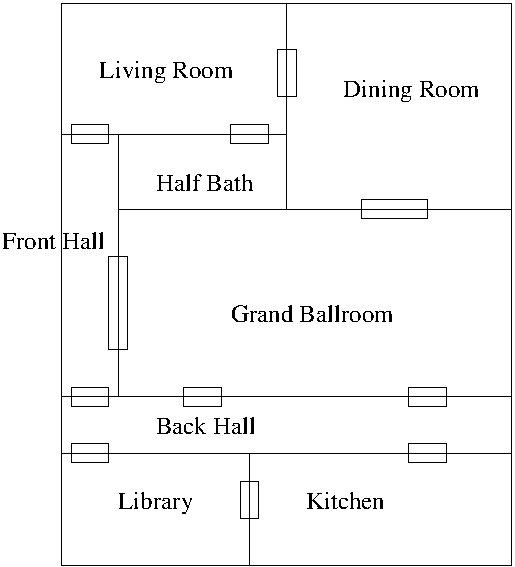
\includegraphics[scale=0.85]{./images/house.pdf}
\n

The agent has the following map of the house, and knows how to move between
rooms. The costs for moving between each pair of rooms with a door connecting
them are listed in the following table.  The costs are the same for the reverse
directions (ie. the cost of going from A to B is the same as the cost of going
from B to A), so only one direction is specified.

\n
\begin{tabular}{|l|l|l|}
  \hline
  & & Cost \\
  \hline
  Living Room & Dining Room & 1 \\
  \hline
  Living Room & Front Hall & 2 \\
  \hline
  Living Room & Half Bath & 1 \\
  \hline
  Front Hall & Back Hall & 1 \\
  \hline
  Front Hall & Grand Ballroom & 3 \\
  \hline
  Dining Room & Grand Ballroom & 2 \\
  \hline
  Back Hall & Grand Ballroom & 2 \\
  \hline
  Back Hall & Library & 1 \\
  \hline
  Back Hall & Kitchen & 2 \\
  \hline
  Library & Kitchen & 2 \\
  \hline
\end{tabular}
\n

The relevant state consists of what room the agent is currently in.  The start
state is the agent being in the library, and the goal is the agent being in the
kitchen.  The actions available to the agent and their costs are defined by the
above table.

\begin{questionList}
\item
Draw a graph of the state-space for this search problem.  Be sure to include and
label all nodes with appropriate names and all edges with the correct weights.

\item
Draw a graph of the search tree that will be created if the agent uses the
Breadth First Search strategy to solve this problem.  Draw only nodes that will
actually be expanded in the course of the search.

\item
Draw a graph of the search tree that will be created if the agent uses the
Uniform Cost Search strategy to solve this problem.  Draw only nodes that will
actually be expanded in the course of the search.

\item
Draw a graph of the search tree that will be created if the agent uses the
Depth First Seach strategy to solve this problem.  Draw only nodes that will
actually be expanded in the course of the search.

\item
With respect to your program implementation, create a table listing the
number of nodes expanded by each search algorithm for each of the gridworld
problems, as well as the approximate runtime (use the \ttt{time} command, and
report \ttt{user} time), and the total cost of the path to the goal that was
found.  Note that timing information is useful only for very rough
relative comparisons, and is not a useful metric for rigorous analysis.  If your
program failed to find a solution, report how it failed.
The table should look something like the following, only with all the maps, and
with the numbers filled in.

\n\noindent
{\small
\begin{tabular}{|l|l|l|l|l|l|l|l|l|l|l|l|l|}
  \hline 
  & \textbf{BFS:} & nodes & time & cost & \textbf{DFS:} & nodes & time & cost & \textbf{A*:} & nodes & time & cost\\
  \hline
  Map 1 & & $x$ & $y$ & $z$ & & $x'$ & $y'$ & $z'$ & & $x''$ & $y''$ & $z''$\\
  \hline
  Map 2 & & $p$ & $q$ & $r$ & & $p'$ & $q'$ & $r'$ & & $p''$ & $q''$ & $r''$\\
  \hline
  . &   & . & . & . &   & . & . & . &   & . & . & .\\
  . &   & . & . & . &   & . & . & . &   & . & . & .\\
  . &   & . & . & . &   & . & . & . &   & . & . & .\\
  \hline
\end{tabular}
}

\item Describe the A* heuristic you chose for the gridworld problems.  Justify its
admissibility and discuss its usefulness in solving these problems, in
particular the later ones.

\item Give an example of a problem where DFS would succeed but BFS would fail.
Describe why this example would cause this behavior.

\item Give an example of a problem where BFS would succeed but DFS would fail.
Describe why this example would cause this behavior.

\item Give an example of a problem where A* will not show improved performance
over BFS.  Describe why this example would cause this behavior.

\item For each of the following heuristics for the gridworld map problems (as
specified in the assignment), state whether the heuristic is admissible, and
then whether it is useful (ie. how good a job does it do of allowing us to
expand as few nodes as possible before finding the goal).  Justify your response. 
\begin{itemize}
  \item $h(n)= $ Euclidean distance from current node to goal node
  \item $h(n)= $ Twice the Euclidean distance from current node to goal node
  \item $h(n)= $ Manhattan distance from current node to goal node
  \item $h(n)= $ Twice the Manhattan distance from current node to goal node
  \item $h(n)= 2$ for all $n$
  \item $h(n)= 0$ if $n$ is the goal, $1$ otherwise
\end{itemize}

\item For a non-planar state-space graph, Euclidean distance is not admissible.
Discuss why this is the case.  Give an example of a real-world problem that
forms a non-planar state-space graph.

\end{questionList}

\end{document}
